\chapter{The Body Surface Potential}


Modelling the atrium itself can provide valuables insight into the effects and
mechanisms of drugs, diseases and inherited conditions as discussed in Chapters 2 and 3.
These simulation studies directly compute the electrical potentials generated by the heart.
However, such measurements are not available to clinical doctors without the
insertion of a catheter electrode or other, more involved, surgical procedures.
Instead they must rely on external tools such as the echocardiogram and the
electrocardiogram (ECG).
To reproduce the ECG with mathematical models, it is necessary to solve what is known as
the ``forward problem''.

\section{The Forward Problem}

To solve the forward problem, Maxwell's equations must be solved to determine the
field in the torso which arises from currents flowing within the heart.
Due to the nature of the problem---the finite size of the torso and the
relatively low frequencies of electrical signals involved---simplifying
assumptions can be made.
The effects of propagation and of capacitive and inductive currents may be
neglected~\cite{Barnard1966}.
The situation must solve therefore becomes a quasi-static volume conductor
problem, which involves only tissue conductances.
The current flow in the torso, $\mathbf{J}$, is given by Ohm's law
\begin{equation}
\label{eqn:bsp:ohm}
\mathbf{J} = \sigma\mathbf{E} + \mathbf{J}^{i}
\end{equation}
where $\mathbf{E}$ is the electric field, $\sigma$ is the tissue conductivity
and $\mathbf{J}^{i}$ is an impressed, or applied, current.
The applied current term is included to allow for the presence of active sources and
is non-zero only at the locations of active sources, i.e. the heart.
Since the total current in (\ref{eqn:bsp:ohm}) is solenoidal (the net flow into or
out of any closed region is zero), thus
\begin{equation}
\label{eqn:bsp:ohm2}
\nabla \cdot \mathbf{J} = 0 = \sigma \nabla \cdot \mathbf{E} + \nabla \cdot \mathbf{J}^{i}
\end{equation}
must be true.
As we are solving the quasi-static problem, $\mathbf{E}$ can be
found from the gradient of the scalar potential, $\phi$, as
\begin{equation}
\label{eqn:bsp:maxwell}
\mathbf{E} = - \nabla\phi
\end{equation}

Substituting (\ref{eqn:bsp:maxwell}) into (\ref{eqn:bsp:ohm2}) then we obtain
Poisson's equation
\begin{equation}
\label{eqn:bsp:poisson}
\nabla^{2}\phi = \frac{\nabla \cdot \mathbf{J}^{i}}{\sigma}
\end{equation}
In an infinite homogeneous conducting medium, a solution to Poisson's equation
for the field at any given point, $\phi$, is~\cite{Plonsey1963}
\begin{equation}
\label{eqn:bsp:infinite}
\phi = \frac{1}{4 \pi \sigma} \int \frac{- \nabla \cdot
\mathbf{J}^{i} }{r} dv
\end{equation}
where $r$ is the (scalar) distance from the elemental volume $dv$ to the point at
which the field is being evaluated.
This is shown in Figure~\ref{fig:bsp:vectors}.
The distance $r$ is the magnitude of the vector $\mathbf{r'}-\mathbf{r}$.


\begin{figure}
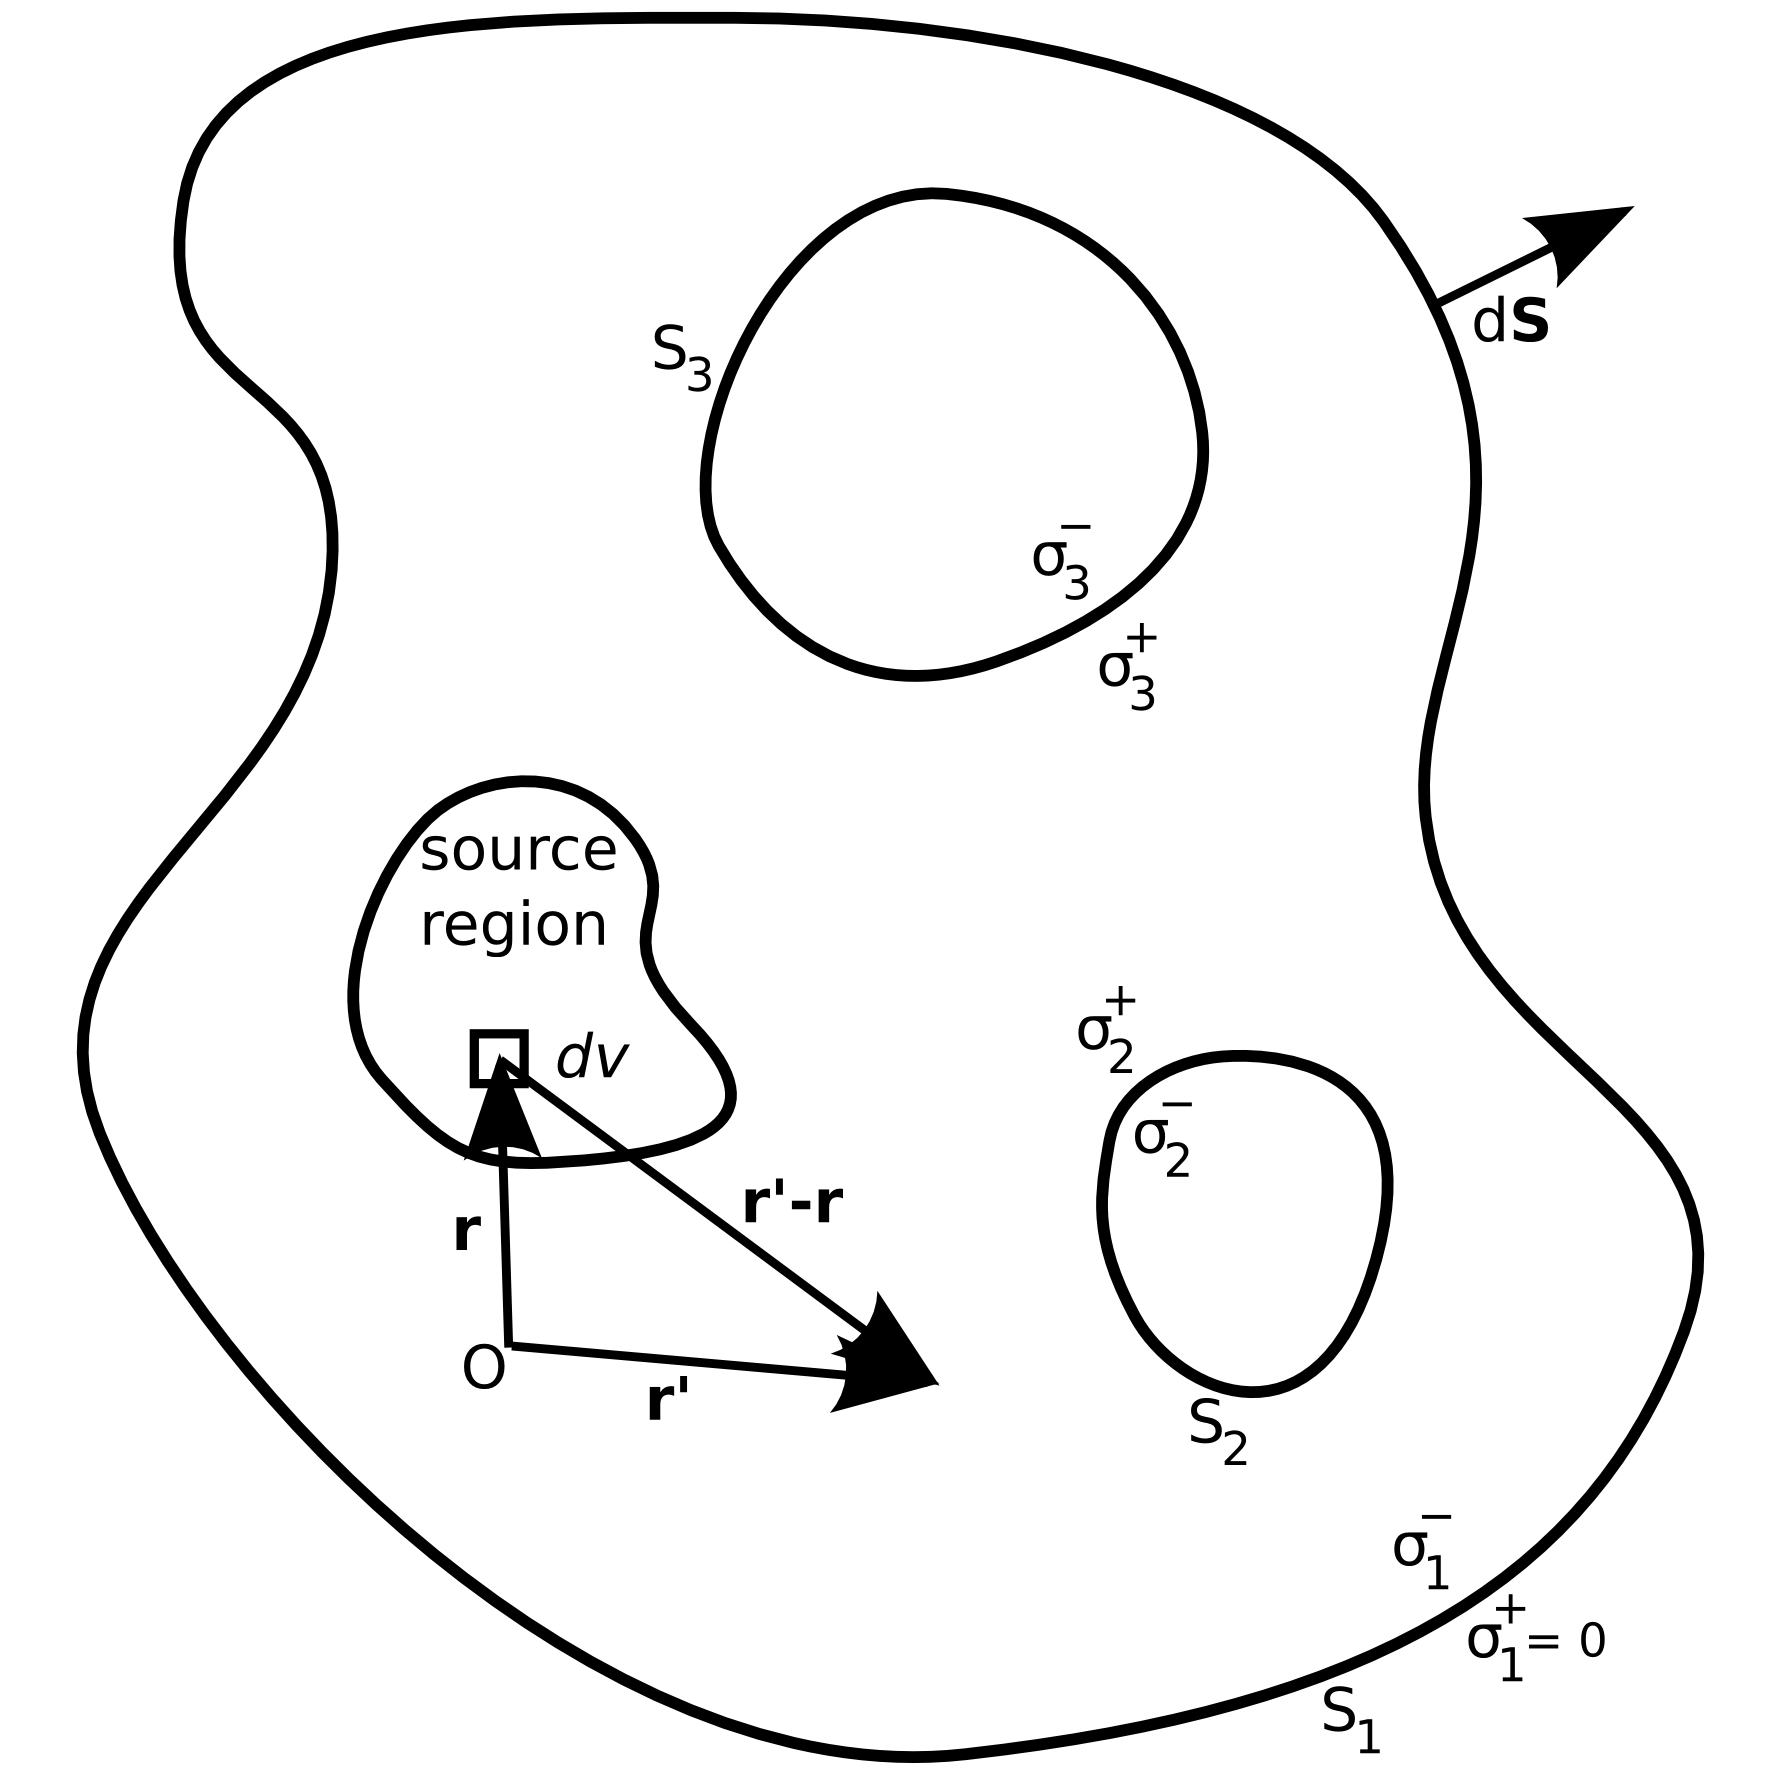
\includegraphics{figures/bsp/bsp_vectors}
\caption[Diagram of the vectors and surfaces involved in the BEM]{
\label{fig:bsp:vectors}
Vectors and surfaces involved in the boundary element method.
The origin is at point $O$.
There are three surfaces shown in the diagram: $\text{S}_{1}$, $\text{S}_{2}$ and
$\text{S}_{3}$.
Each surface has an internal, $\sigma^{-}$ and an external, $\sigma^{+}$,
conductivity.
The $\text{S}_{1}$ surface is the boundary of the region and contains all other
surfaces and dipole sources.
The external conductivity of $\text{S}_{1}$, $\sigma^{+}_{1}$, is therefore zero.
The vector $d\mathbf{S}$ represents an infinitesimal element of the boundary
surface.

The dipole sources are all contained with in the region labelled `source
region'.
The vector $\mathbf{r}$ is a vector to a volume element $dv$ in the source
region.
The vector $\mathbf{r'}$ is a vector to an arbitrary point within the volume
bounded by $\text{S}_{1}$.
}
\end{figure}

To account for the influence of the finite dimensions of the torso we can use
either a FEM or a BEM (See Chapter XXXX for a discussion
of the history of the two methods).
The derivation for the BEM method is based on Green's
Theorem~\cite{Barr1966,Gulrajani1989,Clayton2002},
which states that for a volume, $V$, bounded by a surface, $S$, that
\begin{equation}
\label{eqn:bsp:green}
\int_{V} \left(\phi \nabla^{2}\psi - \psi \nabla^{2}\phi  \right) dv =
\int_{S} \left( \phi \nabla \psi - \psi \nabla \phi \right) \cdot d\mathbf{S}
\end{equation}
where $\phi$ and $\psi$ are scalar functions of position.
If $\phi$ is the electrical potential and $\psi$ is set as $\frac{1}{r}$ where
$r$ is $|\mathbf{r'}-\mathbf{r}|$.
Here, $\mathbf{r'}$ is a vector to an arbitrary point in the volume $V$ at which
we wish to evaluate the field and $\mathbf{r}$ is a vector to an elemental
volume, $dv$, somewhere within the volume $V$.
Using (\ref{eqn:bsp:poisson}) we have
\begin{equation}
\label{eqn:bsp:greenandpoisson}
\int_{V}
    \left(
        \phi \nabla^{2}\left(\frac{1}{r}\right) -
        \frac{1}{r} \frac{\left(\nabla \cdot \mathbf{J}^{i} \right)}{\sigma}
    \right)
dv =
\int_{S}
    \left(
        \phi \nabla \left(\frac{1}{r}\right) -
        \left(\frac{1}{r}\right) \nabla \phi
    \right)
\cdot d\mathbf{S}
\end{equation}

The del operator in (\ref{eqn:bsp:greenandpoisson}) operates on the unprimed (source) coordinates.
Now,
\begin{equation}
\label{eqn:bsp:oneoverr}
\nabla^{2}\left(\frac{1}{r}\right) =
\nabla^{2}\left(\frac{1}{|\mathbf{r'}-\mathbf{r}|}\right) =
-4\pi\delta\left(\mathbf{r'}-\mathbf{r}\right)
\end{equation}
where $\delta$ represents the dirac delta function.  The surface $S$ is the body
surface and so on $S$, $\nabla\phi \cdot d\mathbf{S} = 0$ to a very good
approximation.  (\ref{eqn:bsp:greenandpoisson}) becomes, after substitution and
rearrangement,
\begin{equation}
\label{eqn:bsp:substituted}
\phi\left(\mathbf{r'}\right) =
\frac{1}{4 \pi \sigma}\int_{V} \frac{-\nabla \cdot \mathbf{J}^{i}}{r}dv - 
\frac{1}{4 \pi}\int_{S} \phi\left(\mathbf{r}\right)
\nabla\left(\frac{1}{r}\right) \cdot d\mathbf{S}
\end{equation}

By noting that
\begin{equation}
\label{eqn:bsp:solidanglesubs}
\nabla\left(\frac{1}{r}\right) \cdot d\mathbf{S} =
\frac{\left(\mathbf{r'}-\mathbf{r}\right)}{|\mathbf{r'}-\mathbf{r}|^{3}} \cdot d\mathbf{S} =
d\Omega
\end{equation}
where $d\Omega$ is a differential element of solid angle,
(\ref{eqn:bsp:substituted}) becomes
\begin{equation}
\label{eqn:bsp:substitutedomega}
\phi\left(\mathbf{r'}\right) =
\frac{1}{4 \pi \sigma}\int_{V} \frac{-\nabla \cdot \mathbf{J}^{i}}{r}dv -
\frac{1}{4 \pi}\int_{S} \phi\left(\mathbf{r}\right)d\Omega
\end{equation}
The first term on the right hand side can be recognised as the infinite medium
potential (\ref{eqn:bsp:infinite}) and the second term consists of contributions
from the torso surface.
To discretise (\ref{eqn:bsp:substitutedomega}) we can consider $S$ to be made up of
$n$ triangles, leading to
\begin{equation}
\label{eqn:bsp:discrete}
\phi\left(\mathbf{r'}\right) \approx
\frac{1}{4 \pi \sigma}\int_{V} \frac{-\nabla \cdot \mathbf{J}^{i}}{r}dv -
\frac{1}{4 \pi}\sum_{j=1}^n \phi_{j}\Delta\Omega_{j}
\end{equation}
where $\phi_{j}$ is the potential on the j\textsuperscript{th}\ surface element
and $\Delta\Omega_{j}$ is the increment of solid angle of the
j\textsuperscript{th}\ element when viewed from $\mathbf{r'}$.
To find a solution, Barr et al. noted that $\phi\left(\mathbf{r'}\right)$ is the
potential at an arbitrary point inside $V$.
If these points are chosen to be at the centres of the triangles just inside
the surface $S$ then since $\nabla\phi \cdot d\mathbf{S} = 0$ we can get an
expression for the potential on the i\textsuperscript{th}\ triangle, $\phi_{i}$,
\begin{equation}
\label{eqn:bsp:discretei}
\phi_{i} =
\frac{1}{4 \pi \sigma}\int_{V} \frac{-\nabla \cdot \mathbf{J}^{i}}{r}dv -
\frac{1}{4 \pi}\sum_{j=1}^n \phi_{j}\Delta\Omega_{ij}
\end{equation}
where $\Delta\Omega_{ij}$ is the solid angle of the j\textsuperscript{th}\
triangle seen from the i\textsuperscript{th}\ triangle.
In the summation in (\ref{eqn:bsp:discretei}) there is one term which corresponds to
the case where $i = j$.
In this case, $\Delta\Omega_{ii} = -2\pi$ as from a point just inside $i$, $i$
will obscure an angle of $-2\pi$.  (As a consequence of the vector definition of
solid angle, the solid angle obscured at any point within is negative)
Equation (\ref{eqn:bsp:discretei}) then becomes, after rearrangement,
\begin{equation}
\label{eqn:bsp:discretefinal}
\frac{\phi_{i}}{2} + \sum_{j=1,j \neq i}^n \left(\frac{\Delta\Omega_{ij}}{4\pi} \right)\phi_{j} =
\frac{1}{4 \pi \sigma}\int_{V} \frac{-\nabla \cdot \mathbf{J}^{i}}{r}dv
\end{equation}
which represents a set of $n$ simultaneous equations for the potentials on the
surface elements of the torso.
Using an alternate formulation of (\ref{eqn:bsp:infinite})~\cite{Plonsey1989} in
which $\mathbf{J}^i$ can be considered a dipole density
\begin{equation}
\label{eqn:bsp:b}
B_i = \frac{1}{4 \pi \sigma}\int_{V} \frac{\mathbf{J}^{i}\cdot
\left(\mathbf{r'}-\mathbf{r}\right)}{r^3}dv
\end{equation}
equation (\ref{eqn:bsp:discretefinal}) can be written in matrix form as
\begin{equation}
\label{eqn:bsp:matrix}
\mathbf{A}\mathbf{\phi} = \mathbf{B}
\end{equation}
where $\mathbf{A}$ is a matrix which depends entirely on the geometry of the
torso surface with a typical term of $\displaystyle A_{ij} =
-\frac{\Delta\Omega_{ji}}{4\pi}$ and $A_{ii} = 0.5$, $\mathbf{\phi}$ is a column
vector of the potentials of the $n$ triangles and $\mathbf{B}$ is a column
vector of the infinite medium potentials at the centres of the triangles of the
surface.
Equation (\ref{eqn:bsp:matrix}) can be extended to allow for multiple
inhomogeneities, derivations for which can be found
in~\cite{Barr1966,Geselowitz1968,Geselowitz1970,Gulrajani1983,Gulrajani1989}.

If the surface $S$ was discretised with sufficient accuracy then $\mathbf{A}$
will necessarily be singular, due to the physical nature of the problem.
This was noted by Salu~\cite{Salu1980}\ who proposed a solution which takes
advantage of the physical properties of the system (an alternative method of
removing the singularity of the system was proposed by Lynn and Timlake, the
deflation method).
Salu noted that, experimentally, the potential $\phi$ can only be determined up to
an additive constant.
Therefore $\phi$ can be taken as $0$ at arbitrarily chosen point, without
effecting the general solution.
Assigning $\phi_1 = 0$ in (\ref{eqn:bsp:matrix}) leads to
\begin{equation}
\label{eqn:bsp:salufirst}
\sum_{j=2}^n A_{ij} \phi_j = B_i \quad\quad  i = 1,\cdots, n
\end{equation}
which is a set of $n$ equations in $n-1$ unknowns.
These equations should have exactly one solution.
If an exact solution exists, this implies two things: (a)
(\ref{eqn:bsp:salufirst}) is a set of $n$ consistent equations in $n-1$ unknowns
and (b) the rank of the sub-matrix $A_{ij}: i=2,\cdots,n j=2,\cdots,n$ is $n-1$.
Hence there are $n$ nontrivial $\lambda_i$ such that the rows of $\textbf{A}$
fulfil
\begin{equation}
\label{eqn:bsp:salulambda}
\sum_{i=1}^n \lambda_i A_{ij}  = 0 \quad\quad  j = 2,\cdots, n
\end{equation}
The $\lambda_i$s may be determined up to a proportional factor.
For (\ref{eqn:bsp:matrix}) to be consistent, it is also required that
\begin{equation}
\label{eqn:bsp:salulambdaB}
\sum_{i=1}^n \lambda_i B_i  = 0
\end{equation}
Salu notes that (\ref{eqn:bsp:salulambdaB}) might not hold for a number of
reasons, including numerical inaccuracies in the discretisation of surface or
errors in the calculation of the $B_i$s.
This would lead to a difference between $\phi_{\text{calculated}}$ and
$\phi_{\text{real}}$.
Considering once more the physical properties of the system, $B_i$ as an
electrostatic potential could only be determined up to some additive constant,
$\alpha$.
Equation (\ref{eqn:bsp:salulambda}) then becomes
\begin{equation}
\label{eqn:bsp:salulambdaalpha}
\sum_{i=1}^n \lambda_i \left(B_i+\alpha\right)  = 0
\end{equation}

This can be incorporated into (\ref{eqn:bsp:salufirst}) to get a set of $n$
equations
\begin{equation}
\label{eqn:bsp:salufinal}
\sum_{j=2}^n A_{ij} \phi_j = B_i + \alpha \quad\quad  i = 1,\cdots, n
\end{equation}
Equation (\ref{eqn:bsp:salufinal}) is now numerically consistent and is
equivalent to (\ref{eqn:bsp:matrix}).
Whenever (\ref{eqn:bsp:salulambdaB}) is not fulfilled, due to numerical errors
in the discritisation and creation of $\textbf{A}$ or in the calculation of
$\textbf{B}$, the addition of the $\alpha$ term ensures that
(\ref{eqn:bsp:salufinal}) has a consistent solution.
It is important to note that consistent does not mean necessarily mean accurate
or correct.
The addition of the $\alpha$ term merely ensures that a solution will exist.
Due care must still be taken with the construction of each $A_{ij}$ term and
accuracy can be improved via choosing a finer discretisation for the body
surface mesh.

An efficient solution to the problem of solving the equations and for $\alpha$
was given by Salu.
To do this, we let $\phi_j^* \left(j=2,\cdots,n\right)$ be a solution to the
$n-1$ equations
\begin{equation}
\label{eqn:bsp:saluphijstar}
\sum_{j=2}^n A_{ij} \phi_j^* = B_i \quad\quad  i = 2,\cdots, n
\end{equation}
and let $\phi_j^1 \left(j=2,\cdots,n\right)$ be a solution to the $n-1$
equations
\begin{equation}
\label{eqn:bsp:saluphijone}
\sum_{j=2}^n A_{ij} \phi_j^1 = 1 \quad\quad  i = 2,\cdots, n
\end{equation}
where the $1$ represents a column vector of 1s.
The two vectors $\phi_j^*$ and $\phi_j^1$ both multiply the same matrix,
$\mathbf{A}$ so it need only be inverted once to solve both
(\ref{eqn:bsp:saluphijstar}) and (\ref{eqn:bsp:saluphijone}).
Letting $\phi_j \left(j=2,\cdots,n\right)$ be a solution to the set of $n-1$
equations
\begin{equation}
\label{eqn:bsp:saluphij}
\sum_{j=2}^n A_{ij} \phi_j = B_i + \alpha \quad\quad  i = 2,\cdots, n
\end{equation}
where $\alpha$ is the same alpha introduced in (\ref{eqn:bsp:salulambdaalpha}).
From equations (\ref{eqn:bsp:saluphijstar})--(\ref{eqn:bsp:saluphij}), the
solution to the set of equations will be
\begin{eqnarray}
\label{eqn:bsp:salusolution}
\phi_j&=&\phi_j^* + \alpha\phi_j^1 \quad\quad  j = 2,\cdots, n \nonumber\\
\phi_1&=&0
\end{eqnarray}

Substituting (\ref{eqn:bsp:salusolution}) into the first equation of
(\ref{eqn:bsp:salufinal}) will give
\begin{equation}
\label{eqn:bsp:salualphastep1}
\sum_{j=2}^n A_{1j} \left(\phi_j^* + \alpha\phi_j^1\right) = B_i + \alpha
\end{equation}
or after re-arranging to solve for $\alpha$
\begin{equation}
\label{eqn:bsp:salualphastep2}
\alpha = 
    \frac{
        \left(\sum_{j=2}^n A_{1j} \phi_j^*\right)-B_i
        }{
        1-\left(\sum_{j=2}^n A_{1j} \phi_j^1\right)
        }
\end{equation}
Equation (\ref{eqn:bsp:salualphastep2}) can be used along with
(\ref{eqn:bsp:saluphijstar})--(\ref{eqn:bsp:saluphij}) to solve
(\ref{eqn:bsp:matrix}) to find the body surface potential.

\section{The Atrial Dipole}

In the previous section, the method for solving Maxwell's equations to determine
the body surface potential was derived.
The $\mathbf{B}$ term in the Equation (\ref{eqn:bsp:matrix}) is the infinite
homogeneous medium potential for a number of impressed current sources
$\mathbf{J}^i$.
The model of atrial electrophysiological activity developed in the previous
chapter provides an output of the trans-membrane potentials, $V_m$.
To relate the values of $V_m$ to $\mathbf{J}^i$ we consider the bidomain
model~\cite{Tung,otherguy,Geselowitz1989}.
As previously discussed, the bidomain model considers the cardiac tissue as
comprising two `syncytica' occupying the whole of cardiac tissue and seperated
by the cell membrane.
These are the intra- and extra-cellular spaces.
This leads to the following two relationships
\begin{align}
\label{eqn:bsp:bidomaini}
\mathbf{J}_i & = -\sigma_i \nabla \phi_i \\
\label{eqn:bsp:bidomaine}
\mathbf{J}_e & = -\sigma_e \nabla \phi_e
\end{align}
where $\mathbf{J}$ is a current density, $\sigma$ is the conductivity, $\phi$
is the potential and the subscripts `i' and `e' denote the intra- and
extra-cellular spaces, respectively.
Charge moving from one space to another must cross the cell membrane and is
conserved, leading to the following relationship for $I_m$, the membrane current per unit
volume
\begin{equation}
\label{eqn:bsp:im}
I_m = -\nabla\cdot\mathbf{J}_e = \nabla\cdot\mathbf{J}_i
\end{equation}
By definition the transmembrane potential, $V_m$ is
\begin{equation}
\label{eqn:bsp:tmp}
V_m = \phi_i - \phi_e
\end{equation}
Combining these two equations leads to
\begin{equation}
\label{eqn:bsp:poissonrep}
\nabla\cdot\sigma_i\nabla V_m = -\nabla\cdot\sigma\nabla\phi_e
\end{equation}
where $\sigma = \sigma_i + \sigma_e$, the bulk conductivity of the cardiac
tissue.
Equation (\ref{eqn:bsp:poissonrep}) is of the form of poisson's equation.
The equation can be interpreted to indicate that the term on the left hand side
is the source of the extracellular potentials.
By comparing (\ref{eqn:bsp:poissonrep}) with (\ref{eqn:bsp:poisson}) it is
obvious that
\begin{equation}
\label{eqn:bsp:ji}
\mathbf{J}^i = -\sigma_i\nabla V_m.
\end{equation}

\section{Torso Geometry}

The torso geometry used in this study is shown in Figure~\ref{fig:bsp:torso},A.
It was created by Weixue and Ling~\cite{Lu1993,Weixue1996}\ and has been
used in numerous simulations.
The geometry was derived from CT images of the human torso.
The geometry consists of 412 vertices which were linked by 820 triangular
elements for the thorax and 297 vertices for the for the lungs which were linked
by 586 triangles.
In addition, a geometric representation of the ventricular blood masses was
constructed based on the ventricular mesh from the Weixue and Ling geometry.
This mesh had 295 vertices and 582 elements.
The blood masses of the atria were approximated by a pair of spheres, situated
in the centre of the atrial chambers.
The spheres for the left and right atria each had 162 vertices linked by 320
triangular elements.
These meshes were subdivided using the Blender~\cite{Blender}\ graphical package
into meshes consisting of 13120 elements for the torso, 2344 elements for the
lungs and 2328 for the ventricular blood masses.
Subdividing the meshes in this way did not influence the final form of the ECG
significantly, but did improve the clarity of visualisation of the body surface
potential.
Initial studies using a spherical geometry with a similar number of triangle and
the analytical formula for the potential within a conducting sphere suggest that
the errors~\cite{Ferguson1997} induced through the descritisation are less
than 0.01\%.

\begin{figure}
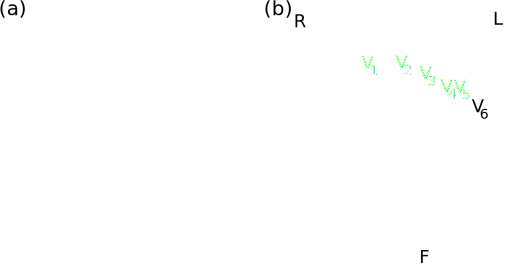
\includegraphics{figures/bsp/thorax_layout}
\caption[Torso showing embedded atrium and lead locations]{
\label{bsp:fig:torso}
\textbf{A} Torso geometry used in this study.
The torso geometry, shown unrefined for clarity is shown as a wireframe.
The lungs are shown in blue, the blood masses in red.
The atrium is visible above the bloodmasses.
\textbf{B} Solid torso geometry showing the locations used for the simulated
electrodes.
}
\end{figure}

The atrial model constructed in the previous chapter was positioned within the
torso using the descriptions of Ho and S\'{a}nchez-Quintana~\cite{Ho2009}
with the ventricular meshes from the original torso used as an additional guide.
First, the model was centred in the atrial co-ordinate system.
Using the z-x-z convention for Euler angles~\cite{eulerref} acting on the heart
(rather than the co-ordinate system of the heart), the atrium was rotated by
$\left(215, 160, 185\right)$.
Following rotation, a translation of $\left(-0.005, -0.08, -0.215\right)$ was
applied to the atrium.
Several of the triangular elements were picked as the sites of the ECG
electrodes.
The electrode locations are shown in Figure~\ref{fig:bsp:torso},B.
Conductances used for the various compartments of the torso are shown in
Table~\ref{tbl:bsp:conductances}.
\begin{table}[h]
    \caption[Conductances of torso compartments]{
        Conductances used for the various compartments of the torso for solving
        the boundary element method~\cite{Seger2004}.
    }
    \begin{tabular}{l r}
     \toprule
     Tissue & Conductivity \\
     \midrule
     Torso & $0.2\,\text{Sm}^{\text{-1}}$ \\
     Lungs & $0.08\,\text{Sm}^{\text{-1}}$ \\
     Blood & $0.6\,\text{Sm}^{\text{-1}}$ \\
     \bottomrule
     \label{tbl:bsp:conductances}
    \end{tabular}
\end{table}

\section{Computational Implementation}

The program which solved the equations and generated the potentials at each of
the elements of the geometry was written in the Fortran 95 programming language.
The $\mathbf{A}$ matrix from (\ref{eqn:bsp:matrix}) was constructed using the
method proposed by van Oosterom and Strackee~\cite{Oosterom1983}\ to
estimate the solid angle subtended by each triangular element.
A subroutine written in C was used to read in the gzip or xz compressed
data files corresponding to each snapshot in time (\ms{1}) generated by the
atrial model.
The impressed current density at each node of the tissue was calculated using
(\ref{eqn:bsp:ji}).
To reduce computational time and memory requirements, the atrial geometry was
divided into 10x10x10 node blocks, around 4000 of which actually had active
nodes within.
The dipoles generated by each active node were aggregated and considered to act
at the centroid of the block determined from the distribution of active nodes
within the block.
These `large' dipoles were then used as the source terms in
(\ref{eqn:bsp:infinite}).
To reduce computation time, the equations were formed into 3 sets of coefficient
matrices, corresponding to the x, y and z components of the radius vector.
These were then multiplied by the relevant dipole components and the results
summed to calculate the potential in the centre of each element.
Decreasing the block size to 5x5x5 nodes had a negligible effect on the computed
body surface potential.
From these dipoles, the $\mathbf{B}$ matrix was calculated.

To solve the resulting set of equations, the LAPACK~\cite{lapack} library was
used.
The $\mathbf{A}$ matrix was factorized using the SGETRF sub-routine.
Numerical experiments determined that only single precision arithmetic was
required.
Solutions calculated using double and single precision showed differences only at
the limits of single precision accuracy--approximately 7 significant figures.
Since the torso is static this need only be done once, at the start of the
calculations.
The SGETRS sub-routine was then used to solve (\ref{eqn:bsp:saluphijone}) and
(\ref{eqn:bsp:saluphijstar}) for each time snapshot using this factorised
matrix.
The zero potential, required for the consistency criterion of Salu, was chosen
to be at element 1 of the mesh.
This element is located at the top of the mesh, at the `neck'.
Generating the body surface potential took one core of horace approximately 60
minutes for \unit{2}{s}\ of atrial activity using the original mesh.
Using the fully refined mesh required approximately 190 minutes for the same
computation.

After computation of the potentials at all points on the body surface, the
results were post-processed to extract the ECG.
These data were stored in a JSON~\cite{json}\ formatted file which contained
arrays representing the voltage of each of the 12 leads, the time step between
each point and, optionally, information on the parameters used by the BSP
algorithm.
JSON offers a lightweight alternative to XML, whilst still being highly readable
without the aid of computer translation.
The high-precision ECG signals, typically at a frequency of \unit{1}{kHz}\
were been passed through a digital low-pass filter at \unit{100}{Hz},
corresponding to the typical frequency response of a clinical ECG unit, from
\unit{0.5}{Hz}\ to \unit{100}{Hz}.
Using the three limb leads (LA, LL, RA) the WCT was computed and used to
contruct isopotential maps.
Whilst the algorithm employed offers a natural zero potential, the use of the
WCT allows for direct comparison with clinical studies which almost exclusively
employ the WCT for this purpose~\cite{Taccardi1966,Mirvis1980}


\section{Simulating Sinus Rhythm}

To simulate the P-wave body surface potential and ECG for the atrium in sinus
rhythm, the atrial model developed in the previous chapter was used.
The simulation of the electrical activity involved the full fibre orientation
description with an anisotropy ratio of 1:9.
There was heterogeneous cell electrophysiology used, with differential
electropphysiology for the atrial myocyte, pectinate muscle and crista
terminalis cells.
The atrium was paced at the site corresponding to the sinus node at a frequency
of \unit{1}{Hz}\ for \unit{2}{s}.
The body surface potential was calculated both with and without the presence of
internal inhomogeneities by setting the internal conductivity of the relevant
compartment to the value in Table~\ref{tbl:bsp:conductances}\ to include that
compartment, or to the torso conductivity to remove its influence.

\subsection{Simulated Body Surface Potential Maps}

The Body Surface Potential Maps (BSPM) were constructed from the output of the
simulations.
In the following descriptions, the distribution is described using the using the
coordinate system of the body rather than of the image.
Note that the raw signals are presented here, that is to say there is no
filtering performed on the signals in the time domain.

\begin{figure}
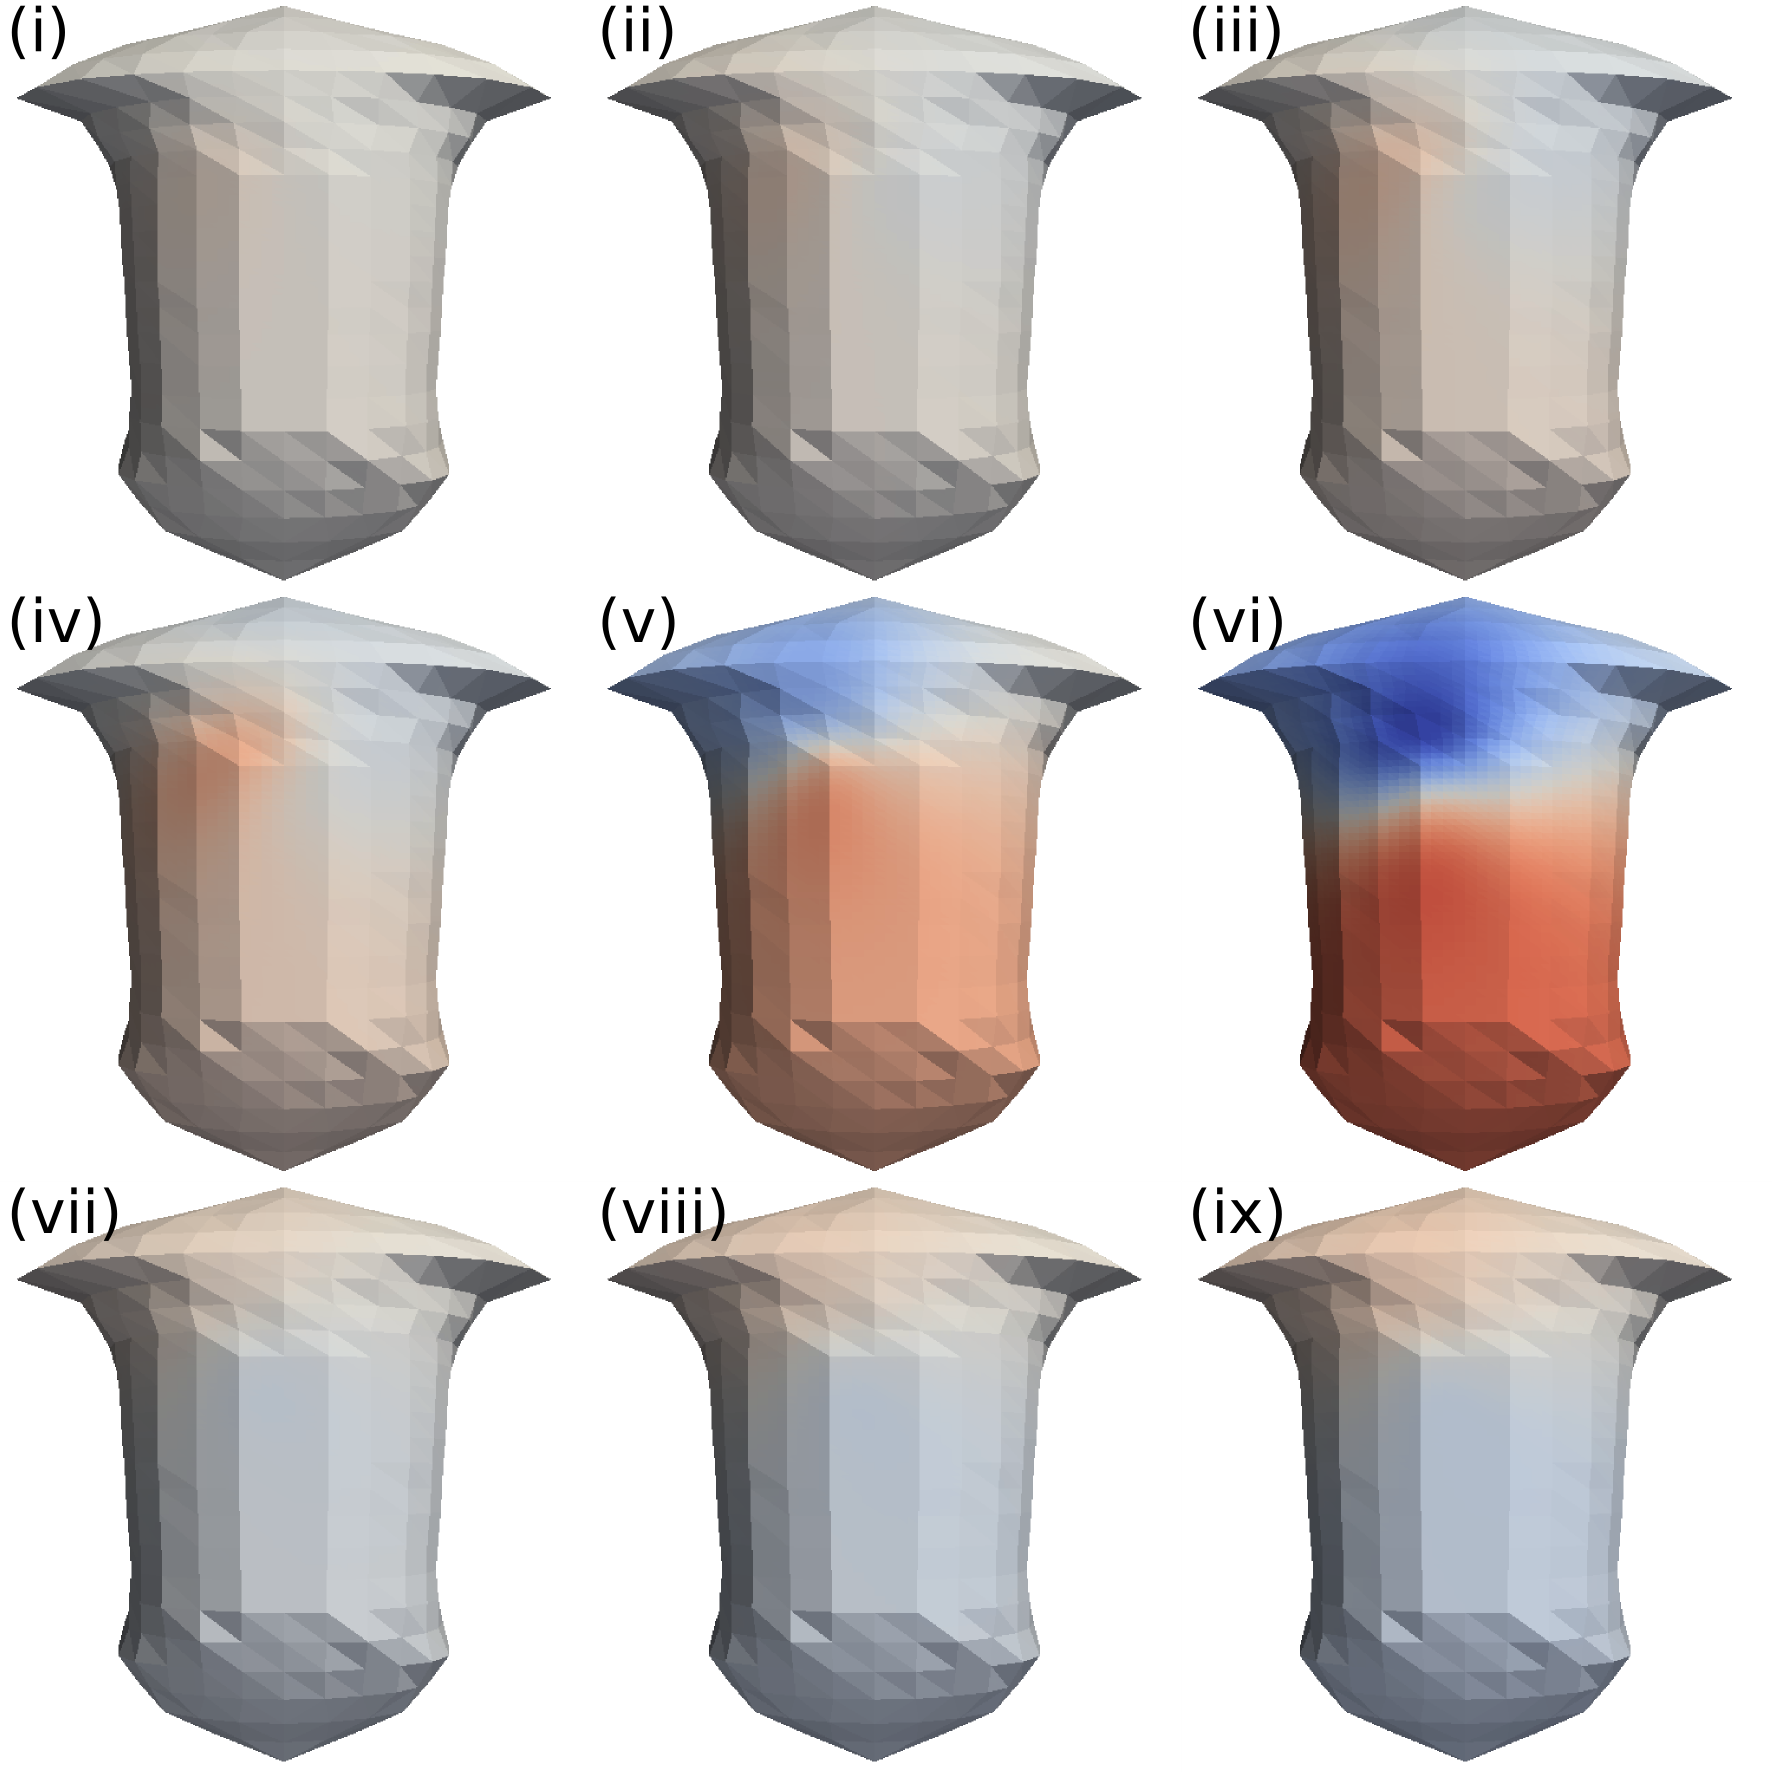
\includegraphics{figures/bsp/bsp_torso}
\caption[Body Surface Potential snapshots, homogeneous torso]{
\label{bsp:fig:homo_bsp}
Simulated BPSM during sinus rhythm with a homogeneous
torso.
The torso begins approximately isopotential before a distinct pattern of
potential, with an area of negative potential over the upper right lung and an
area of positive potential on the left side.
This pattern then reverses during repolarisation.
The maximum potential observed is \mv{0.219}\ and the minimum is \mv{-0.456}.
Snapshots shown for \ms{10}\ (i), \ms{15}\ (ii), \ms{20}\ (iii), \ms{25}\ (iv),
\ms{40}\ (v), \ms{60}\ (vi), \ms{180}\ (vii), \ms{200}\ (viii) and \ms{220}\
(ix)
}
\end{figure}

The evolution of the body surface potential on a homogeneous torso is shown in
Figure~\ref{bsp:fig:homo_bsp}.
The timings of the body surface potential snapshots correspond to the snapshots
of membrane potential shown in Figure~\ref{fig:atrium:validation:main}.
The potential distribution starts off very close to uniform in frame (i) at
\ms{10}\ after initial excitation.
Only excitation and repolarisation wavefronts generate dipoles and in the
initial milliseconds the excitation wavefront is very small.
In \ref{bsp:fig:homo_bsp}(iv) (\ms{25} after initial stimulus) there is an area
of positive potential beginning to appear over the lower right lung, caused by
the rapid conduction along the crista terminalis.
By frames (v) and (vi), the regions of different potential are much more
regularly distributed with a predominately negative region centred on the upper
right lung and a positive region over the lower and left of the torso.
The excitation wavefront is moving towards the left leg.

The three frames (vii--ix) corresponding the to the plateau and beginnings of the
repolarisation show a much more diffuse arrangement of potentials.
The distribution is approximately the mirror image of that seen during
depolarisation, with the predominantly positive regions over the right shoulder.
The diffuse pattern of potentials is caused by the slower repolarisation of
atrial myocytes compared to their depolarisation.
It does not show a disturbance from the smooth pattern as seen for
depolarisation in frame (iv) as the repolarisation is less influenced by the
underlying fibre structure.


\begin{figure}
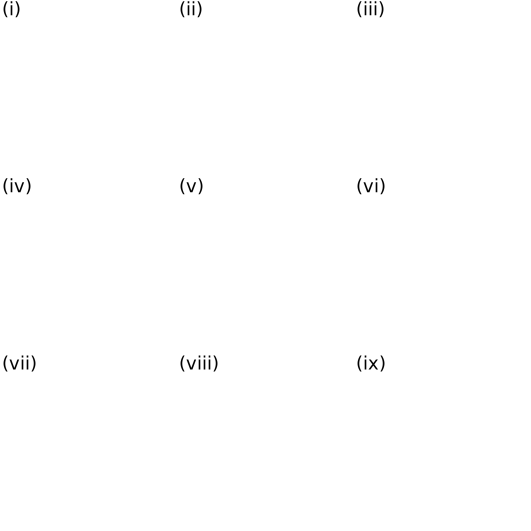
\includegraphics{figures/bsp/bsp_lungs}
\caption[Body Surface Potential snapshots, with lungs]{
\label{bsp:fig:lungs_bsp}
Simulated body surface potential plots during sinus rhythm with lungs assigned
conductivity from Table~\ref{tbl:bsp:conductances}.
The torso begins approximately isopotential before a distinct pattern of
potential, with an area of negative potential over the upper right lung and
area of positive potential on the left hand side.
The area of negative potential is smaller than that seen on during the
homogeneous torso simulations.
This pattern then reverses during repolarisation.
The maximum potential observed is \mv{0.278}\ and the minimum is \mv{-0.449}.
Snapshots shown for \ms{10}\ (i), \ms{15}\ (ii), \ms{20}\ (iii), \ms{25}\ (iv),
\ms{40}\ (v), \ms{60}\ (vi), \ms{180}\ (vii), \ms{200}\ (viii) and \ms{220}\
(ix)
}
\end{figure}

The evolution of the body surface potential with lungs is shown in
Figure~\ref{bsp:fig:lungs_bsp}.
In \ref{bsp:fig:lungs_bsp}(iv) (\ms{25} after initial stimulus) a peak is
beginning to appear over the lower right lung, caused by the rapid conduction
along the crista terminalis but this peak is less pronounced than in the
calculations lacking the lungs.
By frames (v) and (vi), the potential is much more regularly distributed.
In contrast to the simulation without lungs, the region of predominantly
negative potential seems to be higher on the torso and smaller than that seen
without lungs, as is the positive area on the lower left side.
In addition, it appears that the lungs act to give a slight amplification
effect, increasing the ranges of potential seen~\cite{Gulrajani1983}.

The three frames (vii--ix) corresponding the to the plateau and beginnings of the
repolarisation show a much more diffuse arrangement of potentials.
The distribution is approximately the mirror image of that seen during
depolarisation, with the predominantly positive regions over the right shoulder.
The effects of the lungs are almost unnoticeable when compared to the
simulations in the homogeneous torso.

\begin{figure}
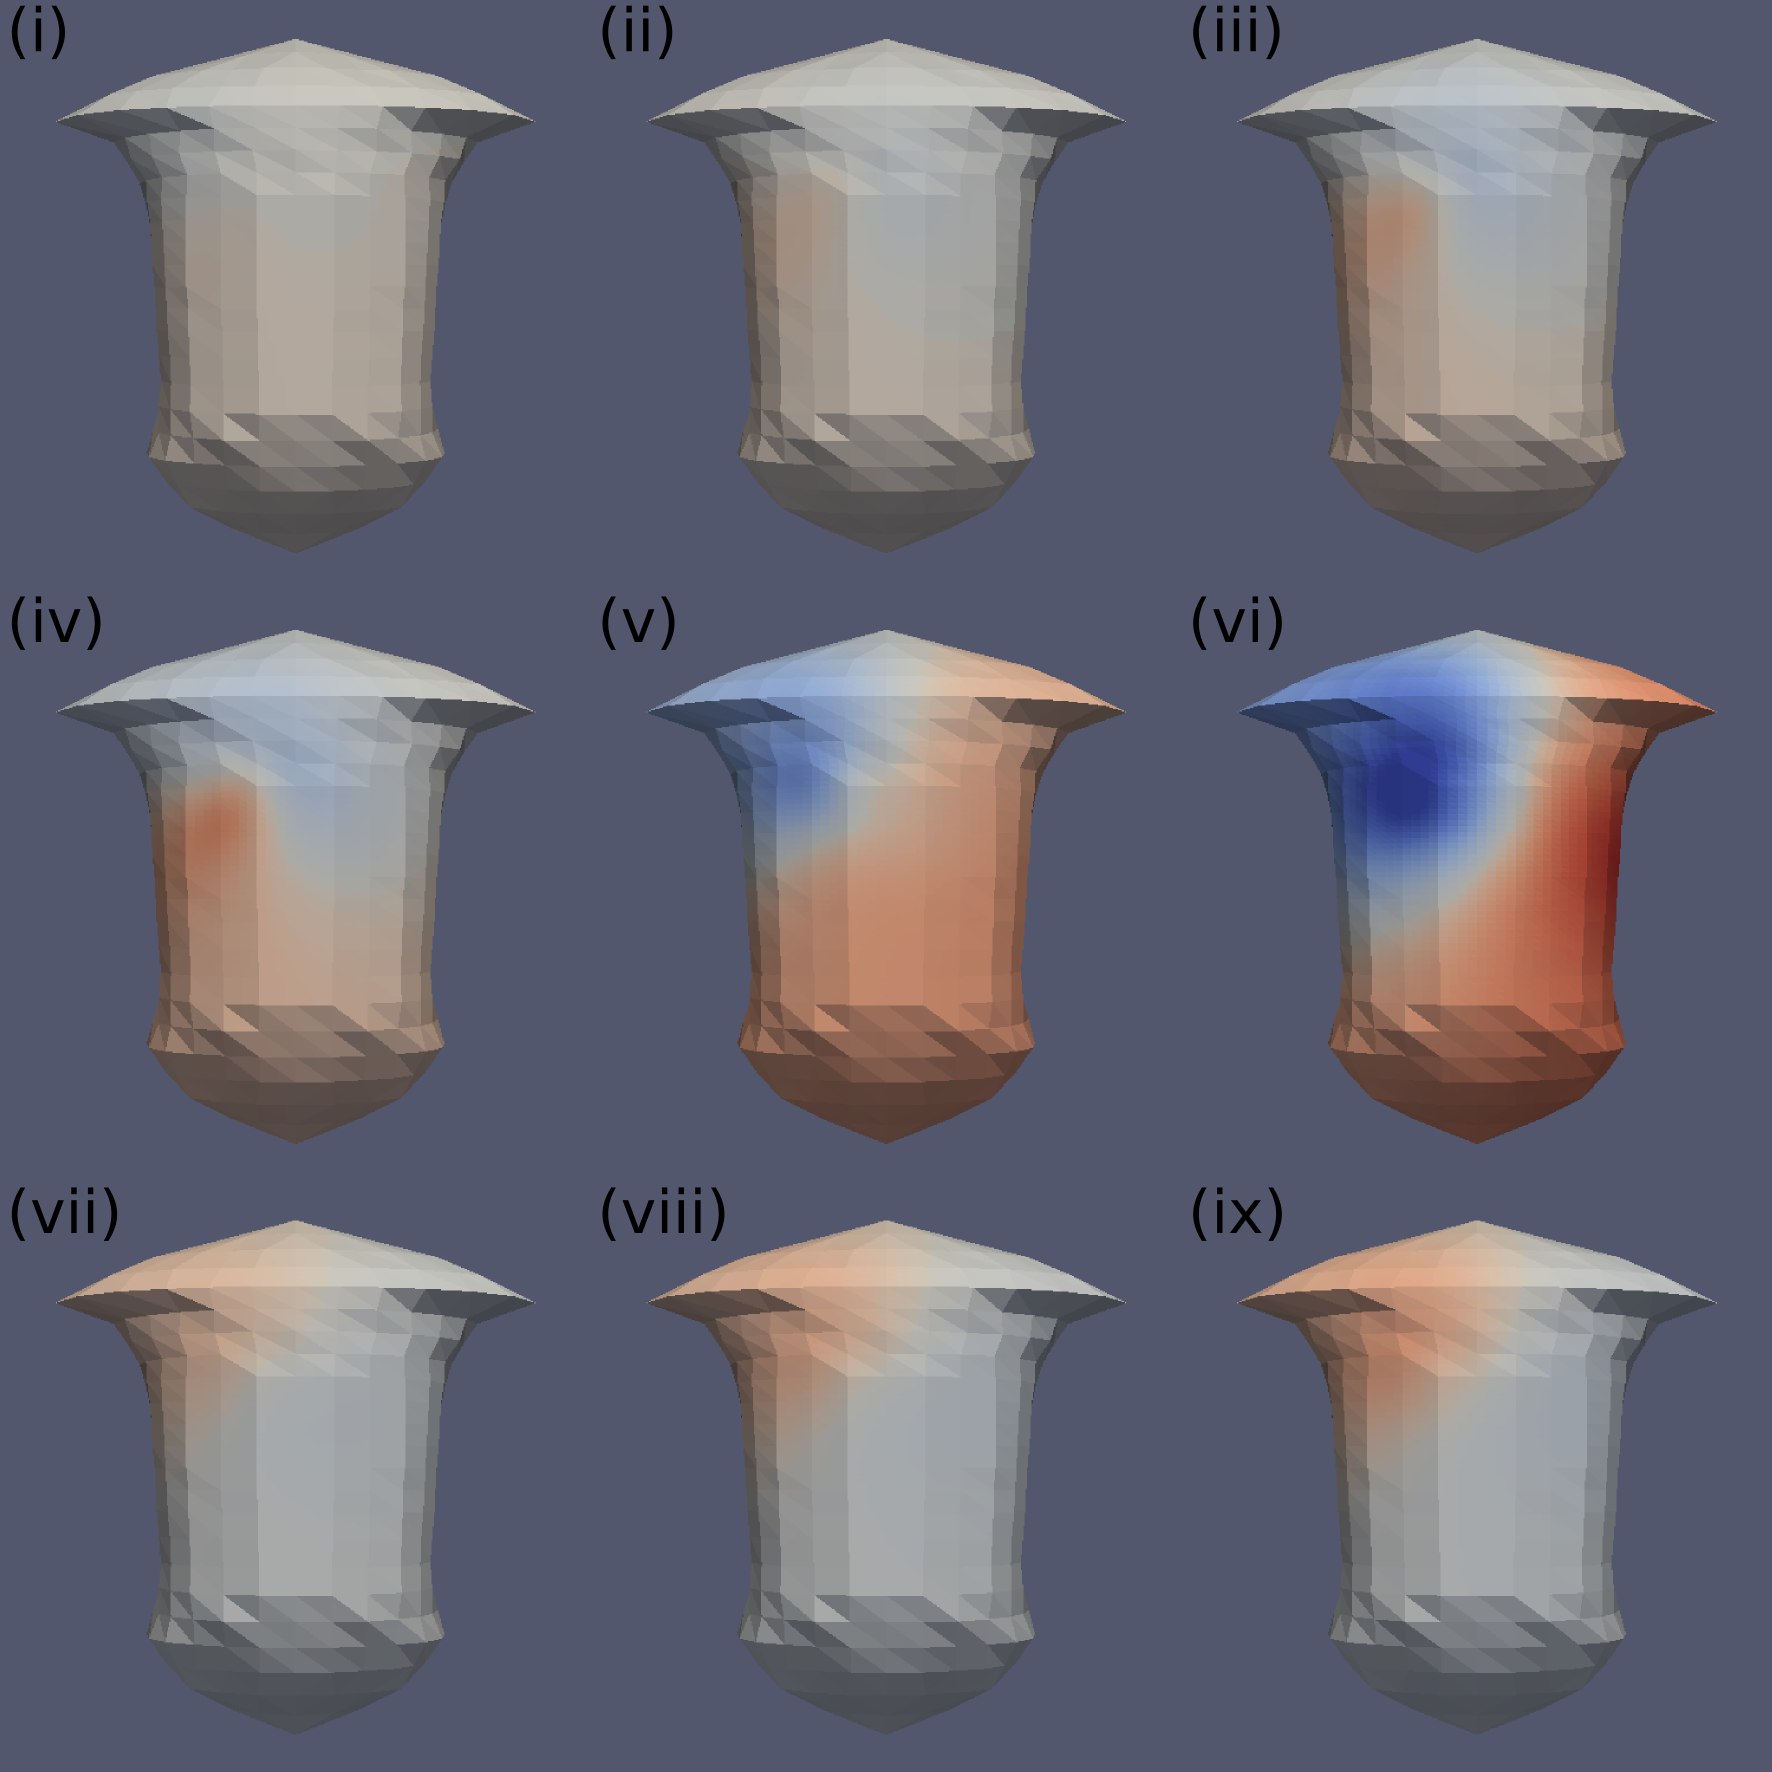
\includegraphics{figures/bsp/bsp_blood}
\caption[Body Surface Potential snapshots, with blood masses]{
\label{bsp:fig:blood_bsp}
Simulated body surface potential plots during sinus rhythm with blood masses assigned
conductivity from Table~\ref{tbl:bsp:conductances}.
The torso begins approximately isopotential before a distinct pattern of
potential, with an area of negative potential over the right shoulder and an
area of positive potential above the left hip.
The pattern of potentials is similar to that observed in the simulation with a
homogeneous torso, but it has a smaller magnitude.
This pattern then reverses during repolarisation.
The maximum potential observed is \mv{0.217}\ and the minimum is \mv{-0.439}.
Snapshots shown for \ms{10}\ (i), \ms{15}\ (ii), \ms{20}\ (iii), \ms{25}\ (iv),
\ms{40}\ (v), \ms{60}\ (vi), \ms{180}\ (vii), \ms{200}\ (viii) and \ms{220}\
(ix)
}
\end{figure}

The evolution of the body surface potential with blood masses present is shown in
Figure~\ref{bsp:fig:blood_bsp}.
The potential distribution is initially almost uniform, when  in frame (i) at
\ms{10}\ after initial excitation.
In \ref{bsp:fig:blood_bsp}(iv) a positive potential is beginning to appear over
the lower right lung, caused by the rapid conduction along the crista
terminalis.
In contrast to the simulations with the lungs present, or in the homogeneous
torso, this appears to have a relatively well defined peak compared with the
more diffuse potential seen in those simulations.
The corresponding negative potential area is more widely spread than in those
cases, extending further down the torso.
By frames (v) and (vi), the pattern of potential observed on the body surface is
very close to that seen in the homogeneous torso, although the maxima and minima
are less extreme in the frames where the blood masses are included.

The three frames (vii--ix) corresponding the to the plateau and beginnings of the
repolarisation show a much more diffuse arrangement of potentials.
The arrangement looks very similar to the corresponding frames from the
homogeneous calculations.


\begin{figure}
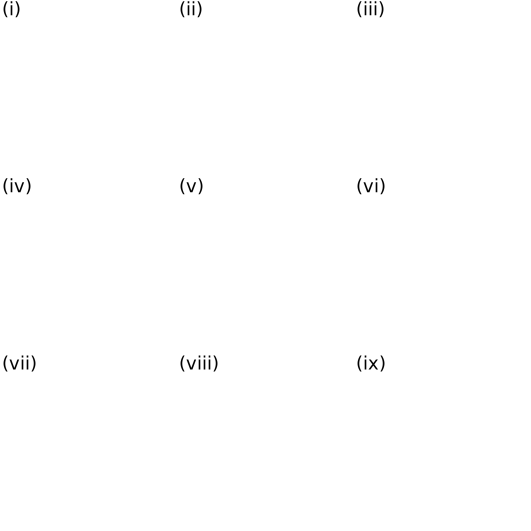
\includegraphics{figures/bsp/bsp_all}
\caption[Body Surface Potential snapshots, with all inhomogeneities]{
\label{bsp:fig:all_bsp}
Simulated body surface potential plots during sinus rhythm with all
inhomogeneties assigned conductivities from Table~\ref{tbl:bsp:conductances}.
The torso begins approximately isopotential before a distinct pattern of
potential, with an area of negative potential over the upper right lung and an
area of positive potential on the left side.
This pattern then reverses during repolarisation.
The maximum potential observed is \mv{0.233}\ and the minimum is \mv{-0.441}.
Snapshots shown for \ms{10}\ (i), \ms{15}\ (ii), \ms{20}\ (iii), \ms{25}\ (iv),
\ms{40}\ (v), \ms{60}\ (vi), \ms{180}\ (vii), \ms{200}\ (viii) and \ms{220}\
(ix)
}
\end{figure}

The evolution of the body surface potential with all inhomogeneities present is
shown in Figure~\ref{bsp:fig:all_bsp}.
In (iv) an isolated peak is beginning to appear over the lower
right lung.
This is closer to the potential distribution shown in the simulations with just
blood masses included than those where lungs are present or where there a
homogeneous torso.
In contrast to this, frames (v) and (vi) show a distribution of potential much
closer to that seen in the simulations where lungs are present, with a smaller
area of negative potential.
The final stages of evolution of the P-wave body surface potential, shown in
frames (vii--ix) show a diffuse pattern, similar to that seen in all the other
simulations.

\subsection{Simulated Electrocardiograms}

In this section, electrocardiograms derived from the BSP distribution are
presented for sinus rhythm.
All of the leads show a minor artifact during the first
$2\text{--}4\,\text{ms}$, due to the stimulation protocol employed.
Disregarding this, the following classifications are used~\cite{kistler2006}.
A positive, or upright, P-wave is one that attains a potential of
$\geq$\mv{0.05}\ and remains above the 0 potential baseline for duration of the
P-wave.
A negative, or inverted, P-wave is one that attains a potential of
$\leq$\mv{-0.05}\ and remains below the baseline for the duration of the P-wave.
A biphasic P-wave is one that is both positive and negative, following the
previous two definitions.


\begin{figure}
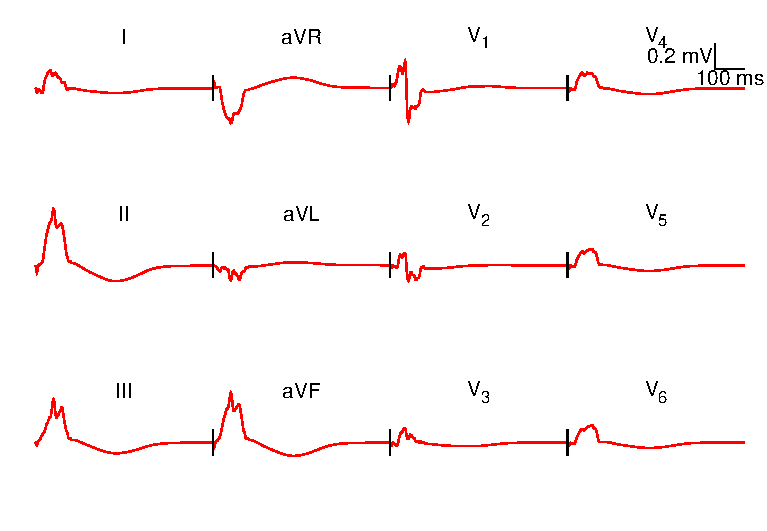
\includegraphics{figures/bsp/ecg_torso}
\caption[12 lead P-wave ECG during sinus rhythm with homogeneous torso]{
\label{bsp:fig:ecg_thorax}
Simulated P-Wave ECG traces during sinus rhythm with homogeneous torso.
One complete action potential cycle is shown.
The stimulus is initiated at $t = 0$ in all traces.
All traces have been smoothed with a \unit{100}{Hz}\ low-pass filter, common to
diagnostic modes on clinical ECG machines.
}
\end{figure}

The ECG derived from the body surface potential simulations with a homogeneous
torso is shown in Figure~\ref{bsp:fig:ecg_thorax}.
The P-wave has a duration of \ms{112}\ in lead II and an amplitude of \mv{0.311}.
The maximum and minimum potential differences observed in the leads are
\mv{+0.311}\ and \mv{-0.359}\ seen in lead II and lead $\text{V}_{1}$, respectively.
The P-wave is upright in leads I, II, aVL, aVF and $\text{V}_{\text{3--6}}$.
It is biphasic in leads III and $\text{V}_{\text{2}}$.
It is inverted in leads aVR and $\text{V}_{\text{1}}$, although there is an small
initial upper deflection in $\text{V}_{\text{1}}$.

The atrial repolarisation wave, the $\text{T}_{\text{P}}$ wave, is easily
visible in all leads except leads III and $\text{V}_{\text{2}}$.
In all the leads in which it appears, it is inverted compared to the P-wave in
that lead and has a lower (less than 50\% in all leads) amplitude.
It appears to start immediately after the P-wave in all leads.
The $\text{T}_{\text{P}}$ is broader than the P-wave, corresponding to the lower
speed of repolarisation.

\begin{figure}
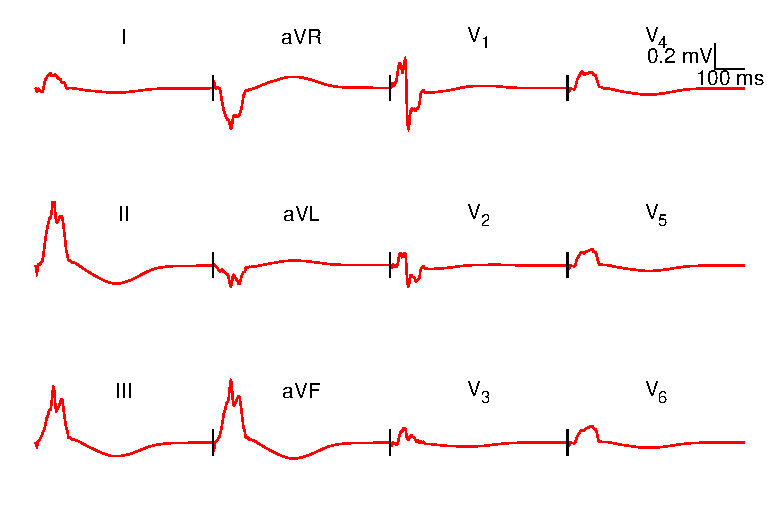
\includegraphics{figures/bsp/ecg_lungs}
\caption[12 lead ECG during sinus rhythm, lungs present.]{
\label{bsp:fig:ecg_lungs}
Simulated P-Wave ECG traces during sinus rhythm with inhomogeneous torso.
Lungs assigned conductivity from Table~\ref{tbl:bsp:conductances}.
One complete action potential cycle is shown.
The stimulus is initiated at $t = 0$ in all traces.
All traces have been smoothed with a \unit{100}{Hz}\ low-pass filter, common to
diagnostic modes on clinical ECG machines.
}
\end{figure}

The ECG corresponding to the simulations with inhomogeneous lungs is shown in
Figure~\ref{bsp:fig:ecg_lungs}.
The P-wave has a duration of \ms{124}\ in lead II and an amplitude of \mv{+0.306}.
The maximum and minimum potential differences observed in the leads are
\mv{+0.306}\ and \mv{-0.390}\ seen in lead II and lead $\text{V}_{\text{1}}$, respectively.
The P-wave is upright in leads I, II, aVL, aVF and $\text{V}_{\text{3--6}}$.
It is biphasic in lead III.
It is inverted in leads aVR and $\text{V}_{\text{1--2}}$, although there are
many of fluctuations visible in lead $\text{V}_{\text{2}}$.
None of this crossed the critical value of \mv{0.05}\ however.
In general the amplitudes of the signals in the leads appears to be lower than
in the simulations without lungs.

The atrial repolarisation wave, the $\text{T}_{\text{P}}$ wave, is easily
visible in all leads except leads III and $\text{V}_{\text{2}}$.
In all the leads in which it appears, it is inverted compared to the P-wave in
that lead and has a lower (less than 50\% in all leads) amplitude.
It appears to start immediately after the P-wave in all leads.
The $\text{T}_{\text{P}}$ is broader than the P-wave in all leads.


\begin{figure}
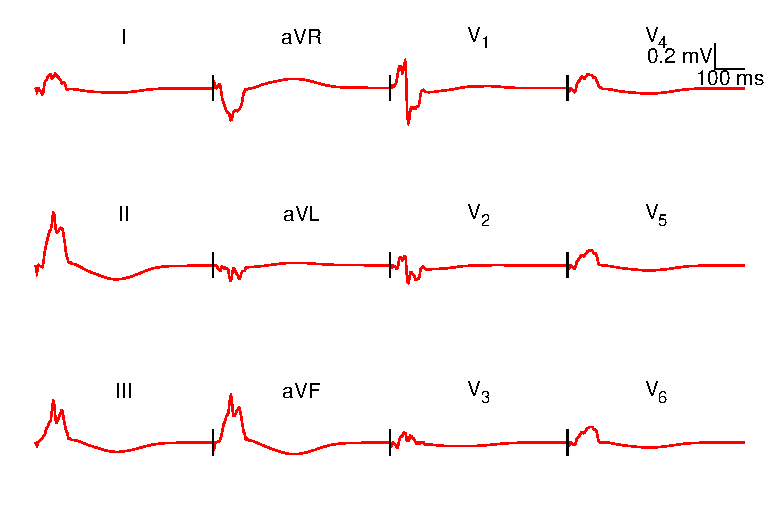
\includegraphics{figures/bsp/ecg_blood}
\caption[12 lead ECG during sinus rhythm, bloodmasses present.]{
\label{bsp:fig:ecg_blood}
Simulated P-Wave ECG traces during sinus rhythm with inhomogeneous torso.
Blood masses assigned conductivity from Table~\ref{tbl:bsp:conductances}.
One complete action potential cycle is shown.
The stimulus is initiated at $t = 0$ in all traces.
All traces have been smoothed with a \unit{100}{Hz}\ low-pass filter, common to
diagnostic modes on clinical ECG machines.
}
\end{figure}

The ECG corresponding to the simulations with inhomogeneous blood masses is shown in
Figure~\ref{bsp:fig:ecg_blood}.
The P-wave has a duration of \ms{126}\ in lead II and an amplitude of \mv{+0.294}.
The maximum and minimum potential differences observed in the leads are
\mv{+0.294}\ and \mv{-0.359}\ seen in lead II and lead $\text{V}_{\text{1}}$, respectively.
The P-wave is upright in leads I, II, aVL, aVF, and $\text{V}_{\text{3--6}}$.
It is biphasic in leads III and $\text{V}_{\text{2}}$.
It is inverted in lead aVR and $\text{V}_{\text{1}}$.

The atrial repolarisation wave, the $\text{T}_{\text{P}}$ wave, is easily
visible in all leads except lead aVL.
In all the leads in which it appears, it is inverted compared to the P-wave in
that lead and has a lower (less than 50\% in all leads) amplitude.
It appears to start immediately after the P-wave in all leads.
The $\text{T}_{\text{P}}$ is broader than the P-wave in all leads.

\begin{figure}
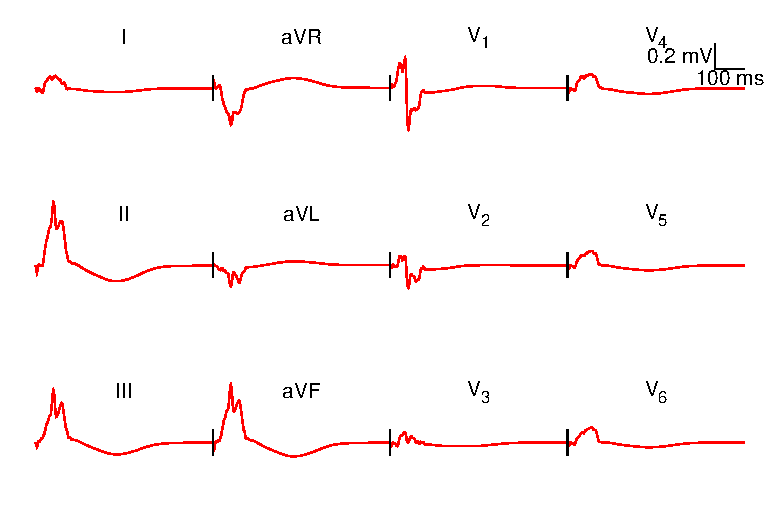
\includegraphics{figures/bsp/ecg_all}
\caption[12 lead ECG during sinus rhythm, all internal inhomogeneities present.]{
\label{bsp:fig:ecg_all}
Simulated P-Wave ECG traces during sinus rhythm with inhomogeneous torso.
Lungs and blood masses assigned conductivity from Table~\ref{tbl:bsp:conductances}.
One complete action potential cycle is shown.
The stimulus is initiated at $t = 0$ in all traces.
All traces have been smoothed with a \unit{100}{Hz}\ low-pass filter, common to
diagnostic modes on clinical ECG machines.
}
\end{figure}

The ECG corresponding to the simulations with all inhomogeneities considered is shown in
Figure~\ref{bsp:fig:ecg_all}.
The P-wave has a duration of \ms{116}\ in lead II and an amplitude of \mv{+0.279}.
The maximum and minimum potential differences observed in the leads are
\mv{+0.279}\ and \mv{-0.385}\ seen in lead II and lead $\text{V}_{\text{1}}$, respectively.
The P-wave is upright in leads I, II, aVL, aVF, and $\text{V}_{\text{3--6}}$.
It is biphasic in lead III.
It is inverted in leads aVR and $\text{V}_{\text{1--2}}$.

The atrial repolarisation wave, the $\text{T}_{\text{P}}$ wave, is easily
visible in all leads except lead aVL.
In all the leads in which it appears, it is inverted compared to the P-wave in
that lead and has a lower (less than 50\% in all leads) amplitude.
It appears to start immediately after the P-wave in all leads.
The $\text{T}_{\text{P}}$ is broader than the P-wave in all leads.

A summary table of the maxima or minima of the leads is shown in
Table~\ref{tbl:bsp:ecg}.
The influence of inhomogeneities on the ECG is perhaps not what would be
expected from the BSPMs.
Whilst the difference between the greatest maximum and the lowest minimum
observed in the leads for the lungs is larger than the difference observed in
the homogeneous torso in agreement with the maximum and minimum potentials
observed on the BSPM, the leads in general have less extreme maxima.
The converse is true for simulations where the blood masses are present.


\begin{table}
    \caption[Maximum and minimum potentials observed in ECG leads]{
        Maximum and minimum potentials observed in the twelve leads of the ECG
        for differing inhomogeneities considered.
        Torso corresponds to the homogeneous case, lungs to the case where the
        lungs are given a conductivity from Table~\ref{tbl:bsp:conductances},
        blood to case where the blood masses were assigned the conductivity from
        Table~\ref{tbl:bsp:conductances} and all, for when both lungs and blood
        masses were assigned differing conductivities.
        For upright and inverted leads, only one potential is given, the maximum
        or minimum potential observed, respectively.
        For biphasic leads, both the maximum and minimum potentials are given.
        All values in mV.
    }
    \begin{tabular}{ l r r r r }
    \toprule
    Lead & Torso & Lungs & Blood & All \\
    \midrule
    I                       & $+0.309$ & $+0.239$ & $+0.287$ & $+0.220$ \\
    II                      & $+0.311$ & $+0.306$ & $+0.294$ & $+0.279$ \\
    III                     & $+0.063$ / $-0.119$ & $+0.104$ / $-0.077$ & $+0.061$ / $-0.134$ & $+0.091$ / $-0.098$ \\
    aVR                     & $-0.310$ & $-0.268$ & $-0.290$ & $-0.249$ \\
    aVL                     & $+0.206$ & $+0.150$ & $+0.206$ & $+0.155$ \\
    aVF                     & $+0.170$ & $+0.202$ & $+0.153$ & $+0.174$ \\
    $\text{V}_{\text{1}}$   & $-0.359$ & $-0.390$ & $-0.358$ & $-0.385$ \\
    $\text{V}_{\text{2}}$   & $+0.074$ / $-0.080$ & $-0.106$ & $+0.051$ / $-0.074$ & $-0.129$ \\
    $\text{V}_{\text{3}}$   & $+0.152$ & $+0.133$ & $+0.156$ & $+0.138$ \\
    $\text{V}_{\text{4}}$   & $+0.169$ & $+0.165$ & $+0.174$ & $+0.159$ \\
    $\text{V}_{\text{5}}$   & $+0.182$ & $+0.173$ & $+0.186$ & $+0.180$ \\
    $\text{V}_{\text{6}}$   & $+0.186$ & $+0.169$ & $+0.181$ & $+0.156$ \\
    \bottomrule
    \label{tbl:bsp:ecg}
    \end{tabular}
\end{table}

The phase of the signal, that is whether it is rising or falling, does not seem
to be influenced by the presence or absence of
inhomogeneities~\cite{Rudy2006,Gulrajani1983}, only the amplitude.
There are exceptions, notably in the $\text{V}_{\text{2}}$ lead, which is either
negative or biphasic depending on the inhomogeneities considered.
Lead III also has distinctly different proportions of the trace above and below
the baseline depending on the inhomogeneities considered.
This has been noted in other studies~\cite{vanDam2005}.
It is again likely to be due to the movement of regions of maximum and minimum
potential caused by the inhomogeneities.
It is possibly more visible with the atria due to the thiner walls and thus
lower mass.

\subsection{Comparisons with Clinical Studies and Information}

The book ``Understanding the ECG'' describes a normal P-wave as being upright in
leads I, II, aVF and $\text{V}_{\text{4--6}}$, as being inverted in aVR and as
being biphasic in III, aVL and $\text{V}_{\text{1--3}}$.
The P-Wave waveforms generated by the combined atrial and torso model are
clearly close to this.
The three Eindhoven leads are in close agreement, as are leads aVR and aVF.
Considering the precordial leads, one can see that the latter three are in good
agreement, whilst the first three show a clear gradation from negative to
positive.
Whether is is due to some subtle flaw in the propagation sequence of the atrial
model, or due to the regions of potential that have developed on the surface
being too focused due to an unconsidered heterogeneity which would further
spread the potential is hard to determine.

Another notable feature is the presence of the $\text{T}_{\text{P}}$ in many of
the leads, which is not normally observed in clinical ECG recordings.
Its presence in the traces generated by this model is due to a combination of
factors.
The first and most obvious reason is that the traces produced by the model are a
lot `cleaner' than those recorded clinically since there are no problems due to
RF interference from wiring, or skeletal muscle activation.
They are also scaled appropriately to view the P-wave, which has an
amplitude which is approximately an order of magnitude smaller than the
QRS-complex which most 12 lead systems are scaled to view.
There is also the lack of the QRS complex, which often obscures the
$\text{T}_{\text{P}}$ wave.

Macfarlane and Lawrie~\cite{MacFarlane1989}\ give the P-wave duration in
lead II for males and females in various age groups.
Due to the hybrid nature of the model, it is hard to know which group gives the
most accurate comparison.
The P-wave duration for the fully inhomogeneous model of \ms{116}\ gives good
agreement with both the $104\,\pm\,12.9\,\text{ms}$ reported for a females of
ages 40--49, which is the age of the heart and with the
$103\,\pm\,14.2\,\text{ms}$ figure reported for males of age 18--29, the age of
the torso.
They report the maximum P-wave potential in lead II to be approximately
\mv{0.23}.
The maximum potential observed in the fully heterogeneous case is \mv{0.28}.
This pattern is repeated for the maximally and minimally observed potentials in
all leads.
This is expected~\cite{Rudy2006,Gulrajani1983,Gulrajani1989,Klepfer1997}\ as internal
inhomogeneities tend to reduce the observed potentials as they `smear' the
electrical signal out over the torso.

Clinical BSPM data for the P-wave has been taken by
Taccardi~\cite{Taccardi1966}\ and Mirvis~\cite{Mirvis1980}.
A comparison of the data taken by Mirvis is shown in
Figure~\ref{bsp:fig:mirvis_compare}.
The BSPM generated by the combined atrial and torso model shows quite good
agreement with the experimental BSPM recorded by Mirvis.
Both sets of data show a solitary maximum point which emerges approximately in
in the centre of the chest and then moves off to the left (torso co-ordinates),
with an area of negative potential which appears over the right chest.
By the time of the peak of the P-wave (\ms{48--68}), there is a positive peak
lying over leads $\text{V}_{\text{4--6}}$, which remains there until the P-wave
starts to end (\ms{80--90}).
During the latter stages of the P-wave, there is a negative potential over the
centre of the chest and the first and second precordial leads.
The agreement is not perfect, however.
The potentials attained in the model are much higher than those noted by Mirvis
or Taccardi.
In addition the distribution of the potentials, particularly in frames
\ms{24--48}\ appears to suggest that the cardiac axis of the model would ideally
be rotated to lie in a more frontal direction.

\begin{figure}
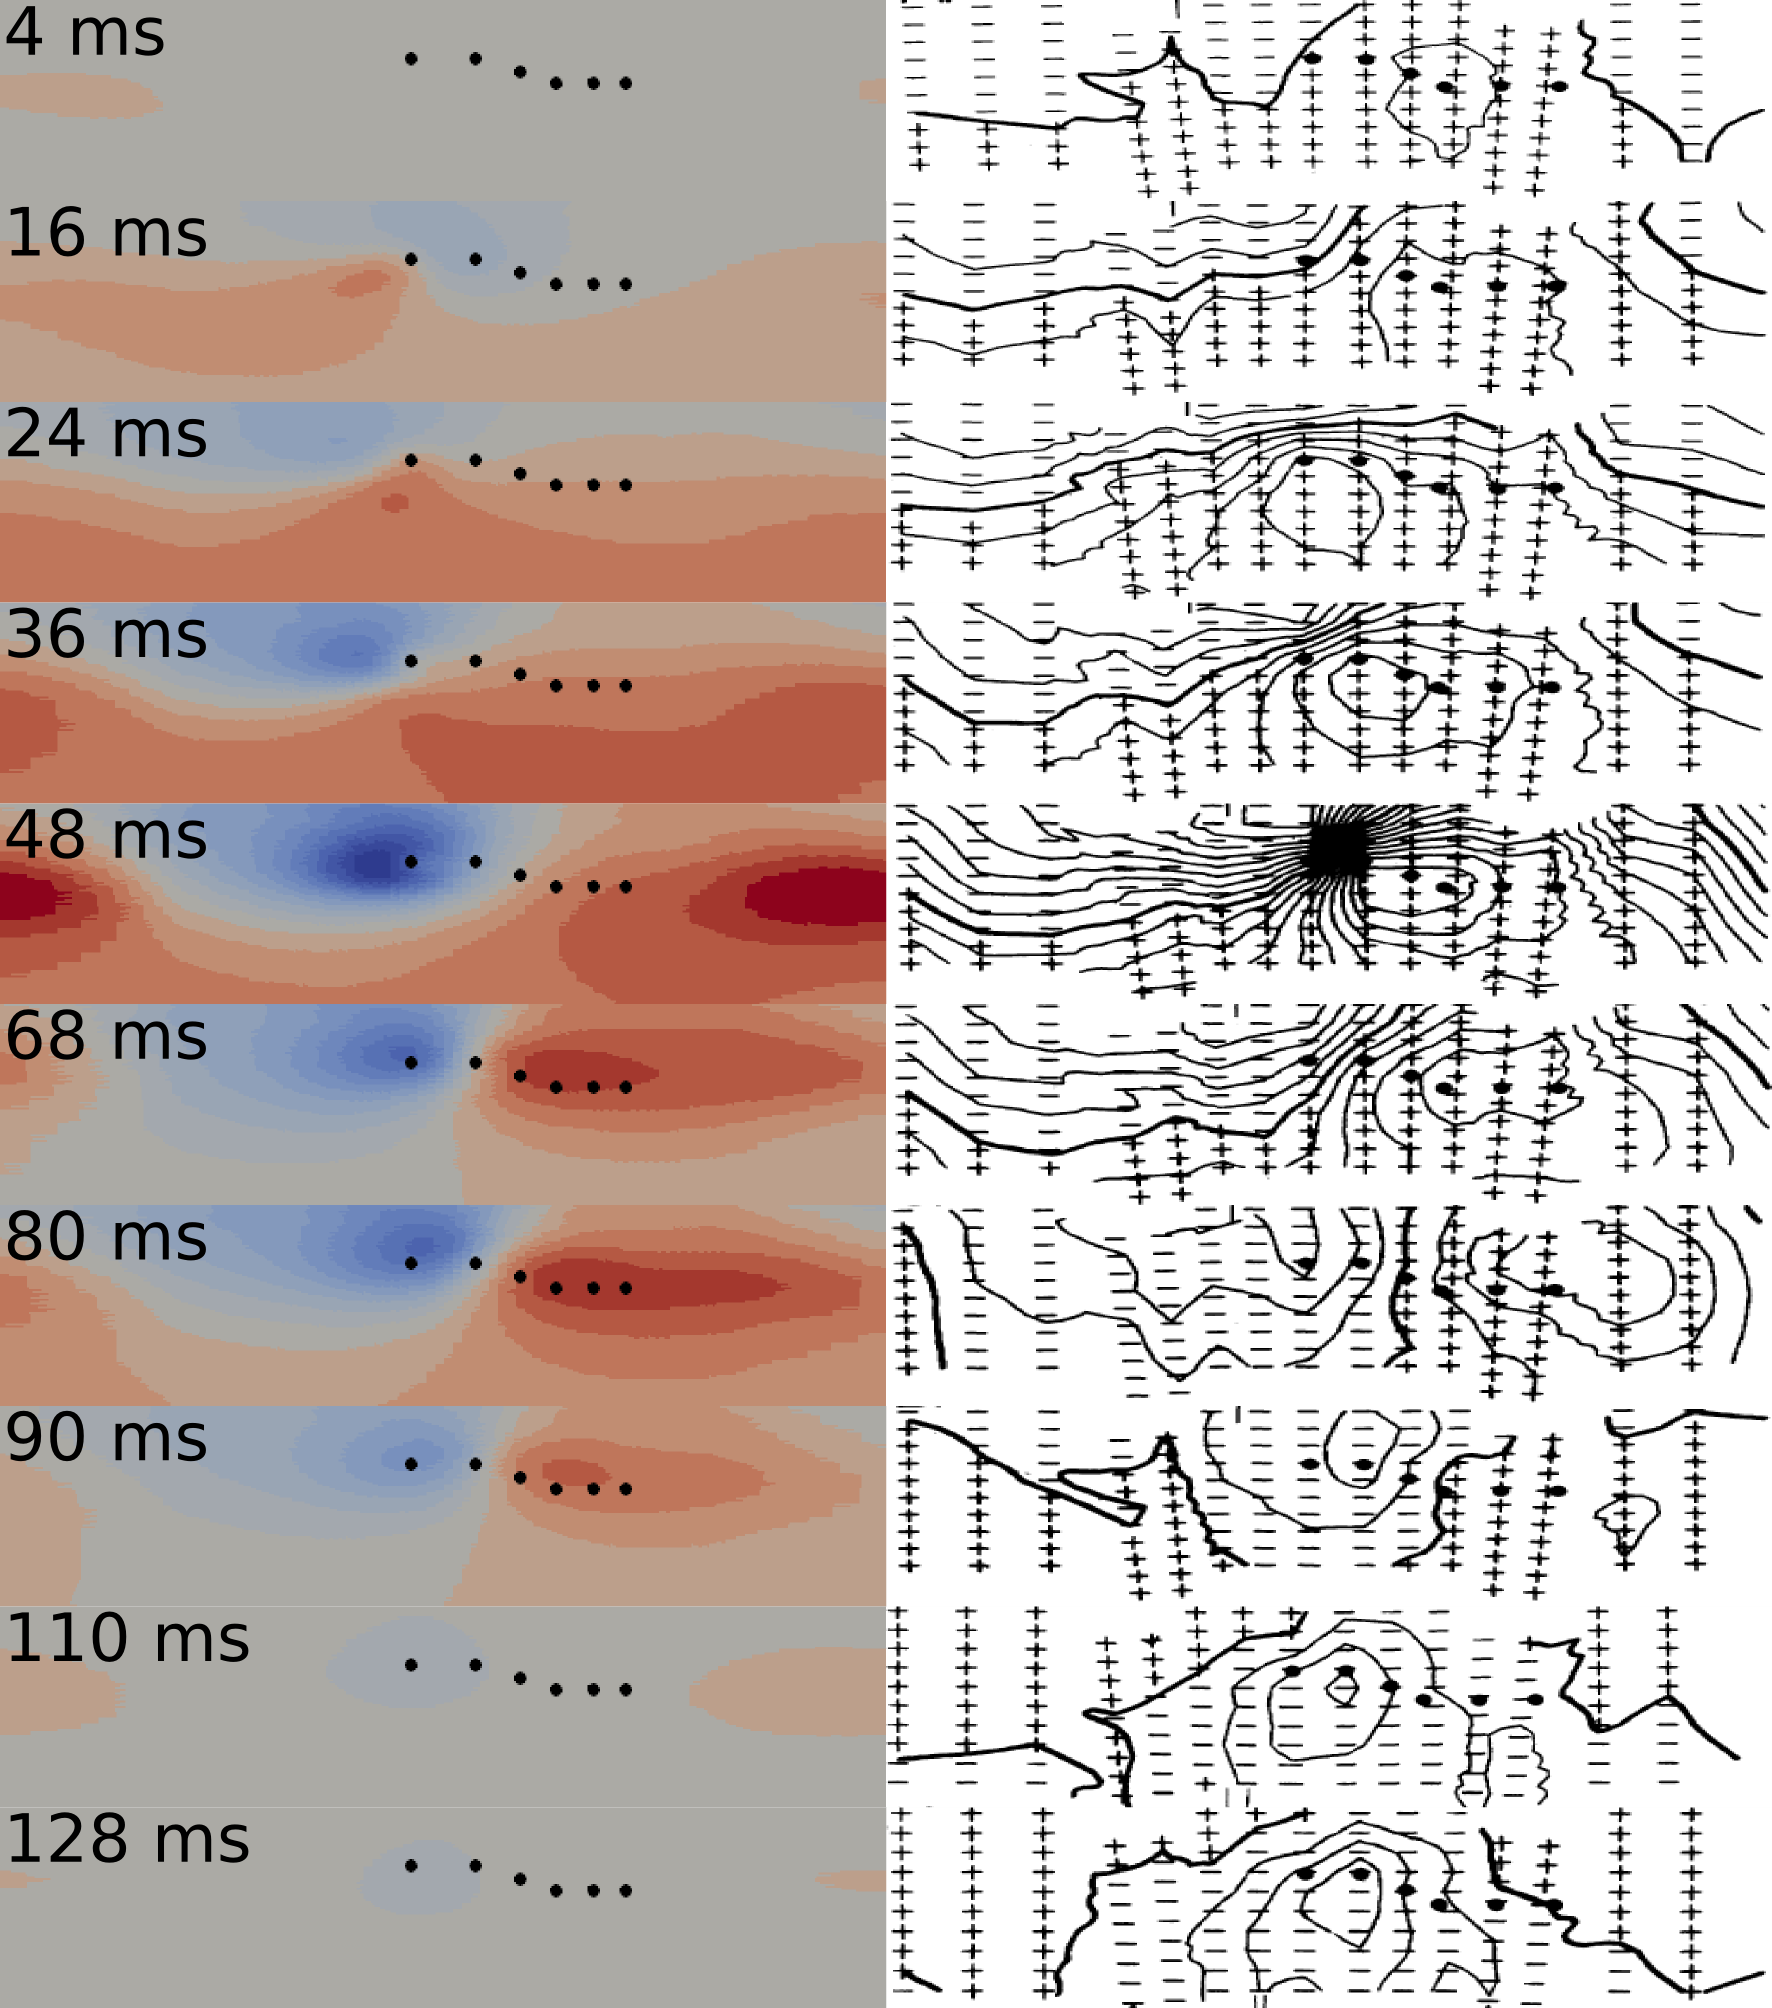
\includegraphics{figures/bsp/mirvis_compare}
\caption[Comparative BSPM from the fully inhomogeneous model and Mirvis]{
\label{bsp:fig:mirvis_compare}
BSPMs generated by the combined torso and heart model (left) compared with
clinical BSPM data recorded by Mirvis~\cite{Mirvis1980} (right).
Precordial leads are shown as black circles (both sides).
On the left, red indicates increasingly positive potentials, blue increasingly
negative and Grey indicates a potential near zero.
On the right, $+$ and $-$ signs indicate regions of positive and negative
potentials, respectively.
Zero potential is the bold contour, other contours in \mv{0.01}\ intervals.
All potentials relative to the Wilson's Central Terminal.
The snapshots of the BSPM are from the indicated times, relative to the start of
the P-wave.
Right hand panels adapted from Mirvis~\cite{Mirvis1980}, Figures 2--4.
}
\end{figure}

\subsection{Comparisons with other Modelling Studies}

Modelling studies of the P-wave BSP are relatively rare in the literature with
the vast bulk of studies concerning themselves with the ventricles.
There have been several
studies~\cite{Lian2002,Seger2004,Oosterom2005,vanDam2005} which have considered
the generated P-wave.
These studies represent a range of approaches to the problem.

The Lian et al.~\cite{Lian2002}\ study used the Weixue~\cite{Lu1993,Weixue1996}\ torso
geometry as in this study.
Their source model was based on atrial geometry extracted from the original CT
images the torso surface was also based on.
It was discretised at a resolution of \mm{1.5}.
Electrical activation of each of the 65,000 nodes was determined using a rule
based~\cite{Lu1993}\ system, similar to cellular automata, although a full
electrophysiological model was used at each point.
The activation sequence of the nodes is predetermined and there is no direct
coupling between cells.
For calculation of the BSP, the nodes are assigned to one of 29 dipole blocks.
The Lian et al. model is very simplistic, but can never-the-less reproduce the
broad detail of the P-wave BSPM.
They see a similar distribution of potential, although their maps show a very
simple distribution of potential without the complexities visible in both the
BSPMs generated by the model described in this chapter and seen in the data from
Mirvis~\cite{Mirvis1980}.

Seger et al~\cite{Seger2004}\ used a finite element approach to compute the
P-wave BSPM in both sinus rhythm and with clockwise and counter-clockwise AF.
Their atrial model and the torso model were extracted from MRI data.
Propagation in the atrial model used a 3 state cellular automaton model for the
membrane potentials, but used a complex distribution of conduction velocities.
Calculation of the BSPM considered heterogeneous lungs and blood masses, as well
as anisotropic conduction within the atria itself.
Their P-wave duration and BSPM show a very similar distribution of potentials to
that observed in this chapter.
They report that the maximum and minimum potentials observed are approximately
\mv{0.25}\ and \mv{-0.25} respectively--similar in magnitude to those observed
in this model.
The use of a cellular automaton model would make simulation of Ischemia, genetic
mutation or atrial fibrillation induced remodelling problematic.

Oosterom et al.~\cite{Oosterom2005}\ used a technique called the Equivalent
Double Layer~\cite{Huiskamp1988} (EDL).
Briefly, this technique uses Gauss' Theorem to represent the dipole generated by
the whole atria using the voltage distribution on the surface of the atria.
The validity of this technique under all conditions has been questioned both
theoretically~\cite{Geselowitz1992}\ and experimentally~\cite{Scher1994}.
Their torso and atria are based on MRI data.
The atrial model is generated from the endocardial surface of the atria.
The atrial walls are then assumed to have a uniform thickness of \mm{2},
extending out from the endocardial surface in all directions.
Membrane kinetics within this volume use a modified version of the Courtemanche
et al.~\cite{CRN98}\ model, modified to have a shorter \apd\ which was
optemized based on recorded potentials from the patient who provided the MRI
geometry.
They do not present BSPMs from their simulations, though their optemized results
show very close agreement with the recorded clinical ECGs from the study.

Van Dam et al.~\cite{vanDam2005}\ also use the EDL for their BSP calculations.
They used a similar model that of Oosterom et al.~\cite{Oosterom2005}, though in
this case it was entirely derived from one patients MRI dataset.
They used the model to investigate the effects of including or removing internal
inhomogeneities.
They noticed different effects (both qualitatively and quantitatively) on the
ECG leads to the study in this chapter.
The reasons for these differences are unclear due to the complexities of both of
the involved models.
One possible reason is the difference in the relative size of the atria to the various
inhomogeneities.
The van Dam model has a much lower atrial tissue mass as it has walls of uniform
thickness, whilst the anatomical model used in this chapter has non-uniform
walls which are generally thicker than \mm{2}.
However, they agree in the need for the inclusion of such inhomogeneities.

\section{Limitations of the Model}

Whilst the presented model of the human atrium and torso provides a relatively
good reproduction of the features of the body surface potential distribution and
ECG, it does omit several factors that could be considered.
There were also compromises made due to the `assembled' nature of the model.
It is possible that a `better' orientation for the atrium could be found, due to
the scarcity of anatomical landmarks present in the torso for the study to guide
its placement.
The model of the blood masses, particularly those of the atria could be improved
to more realistically model the shape, perhaps by basing the outer surface of
the blood masses off a mesh extracted from the epicardial surface.
The size and shape of the ventricular bloodmasses, whilst extracted from the
internal surfaces of the ventricular mesh associated with the torso, do not
exactly correspond to the sizes of the atrial valve openings.
In addition, the presence of the lungs presented a constraint on the location of
the atria, due to a requirement that the atrium should reside wholely within the
main torso cavity--an orientation that had previously been considered `good' had
to be discarded when lungs were introduced.

The model considers only a few internal inhomogeneities, the lungs and the blood
masses.
Other inhomogeneities such as the skeletal muscle layers and subcutaneous fat
have not been included, although previous simulation studies suggest their
influence is small~\cite{Klepfer1997}.
However the smaller mass of the atria might make their influence more
significant~\cite{vanDam2005}\ and so this factor might need further
investigation.
In addition, the anisotropic nature of cardiac muscle was only considered during
the calculations of the electrical propagation, it was not considered during the
computation of the dipole sources of the heart.
What influence this has is unknown, as only one computational study of the
atrial excitation appears to have considered it~\cite{Seger2004}\ and then not in
isolation.

The model considers coupling only in one direction; the heart potential
distribution drives the torso potential distribution.
A more complete study might consider coupling in the other direction as well.
This would require significant changes to the model, necessitating a bidomain
approximation to be used for the propagation and a finite difference or finite
element formulation used for the torso.

Finally, the model is completely static.
There is no consideration of the contractile nature of the myocardium.
This would have influence both on the pattern of propagation and the distance
between dipole locations and the boundary elements.
The contractile cycle would also influence the spatial distribution of the
blood masses.
This would significantly increase the amount of computational power required to
solve the problem, but would not be impossible with the current generation of
computers.

\section{Conclusions}

A model capable of reproducing the P-wave body surface potential has been
produced.
The model is based on a realised atrial geometry which includes both anisotropic
conduction and heterogeneous electrophysiology.
The atrial model is embedded in a torso which was derived from CT images.
The torso features regions of inhomogeneous conductivity, representing the blood
masses of the heart and the lungs.
The effects of including or removing these inhomogeneities has been
investigated.
Their presence is found to generally improve the quality of the generated ECG,
making the generated potentials closer to physiological values.
The complete model has been validated by comparison with both other computer
models and with clinical data.

The model is the start of a tool for investigating many diseases of the atria
and the effect they have on the ECG and BSPM.
Since it is based on the Courtemanche atrial myocyte model, a biophysically
detailed second generation model, it can be used for the investigation of a
broad spectrum of effects, including both conduction defects and the complex
electrophysiological changes induced by both genetic mutation and atrial
fibrillation.
